% Belief-updating microfoundation for the partial-adjustment dynamics.
% Slotted into model.tex as a subsection of Section \ref{sec:mech}.
% Provides the structural counterpart to the reduced-form fiscal-illusion
% mechanism presented in Section \ref{sec:fiscal_illusion}.

\subsection{Belief-Updating Microfoundation} \label{sec:belief_updating}

The dynamics presented in Section \ref{sec:mod_results} were generated by both a perfect-foresight (PF) algorithm and a partial-adjustment (PA) algorithm. The PF run delivers the rational-expectations capitalization benchmark of Section \ref{sec:fiscal_illusion}: a near-immediate jump in $p_{h,t}$ at the moment the maintenance shock is realized. The PA run delivers the gradual price decline that matches the empirical event-study path. In its bare form, however, the PA algorithm is an ad hoc smoothing device. The purpose of this subsection is to derive the same partial-adjustment dynamics from an explicit Bayesian signal-extraction problem on the road-capital stock $G_t$, thereby providing a microfounded alternative to the rational-expectations benchmark and tying the structural friction parameter to a primitive observability cost.

\subsubsection{Information Environment}

Households continue to choose consumption $c_t$, housing $h_t$ and labor $n_t$ subject to the budget constraint and Euler conditions derived earlier. The only modification is that they do not directly observe the road-capital stock $G_t$ that enters the amenity function $A(G_t)$. Instead, at each date $t$ they observe a public signal
\begin{equation}
s_t \;=\; G_t \;+\; \varepsilon_t,
\qquad \varepsilon_t \sim \mathcal{N}(0,\,\sigma_t^2),
\label{eq:signal}
\end{equation}
together with the realized law of motion for the fiscal instrument $\tau_{h,t}$ and the level of last period's maintenance $M_{t-1}$. The noise variance $\sigma_t^2$ is a decreasing function of the gross change in physical road condition:
\begin{equation}
\sigma_t^2 \;=\; \frac{\bar{\sigma}^2}{1 + \omega \,\big|\,G_t - G_{t-1}\,\big|},
\qquad \omega > 0.
\label{eq:visibility}
\end{equation}
Equation \ref{eq:visibility} captures the visibility channel emphasized in Section \ref{sec:fiscal_illusion}: when the underlying capital stock barely moves, residents and prospective buyers have little observational basis to distinguish ``well-maintained'' from ``under-maintained'' jurisdictions, so the noise variance is high. Once physical decay becomes large enough to register visually --- in our setting, once the fine-tuned ConvNeXt classifier in Section \ref{sec:data} would re-classify the surface --- the noise variance collapses and the signal becomes informative.

Households form a posterior $\hat{G}_t \equiv \mathbb{E}[\,G_t \mid \mathcal{I}_t\,]$ over the latent road-capital stock conditional on the information set $\mathcal{I}_t = \{s_t, s_{t-1}, \dots, \tau_{h,t}, \tau_{h,t-1}, \dots\}$. Standard Kalman filtering on Equations \ref{eq:signal}--\ref{eq:visibility} together with the law of motion for $G_t$ in Equation \ref{eq:roads} yields the recursive updating rule
\begin{equation}
\hat{G}_{t} \;=\; \hat{G}_{t \mid t-1} \;+\; \mathcal{K}_t \,\big(s_t - \hat{G}_{t \mid t-1}\big),
\qquad
\mathcal{K}_t \;=\; \frac{P_{t \mid t-1}}{P_{t \mid t-1} + \sigma_t^2},
\label{eq:kalman}
\end{equation}
where $\hat{G}_{t \mid t-1}$ is the one-step-ahead forecast, $P_{t \mid t-1}$ is the prior variance, and $\mathcal{K}_t \in [0,1]$ is the Kalman gain. When the signal is uninformative ($\sigma_t^2 \to \infty$, equivalently $|G_t - G_{t-1}|$ small), $\mathcal{K}_t \to 0$ and the posterior tracks the prior. As physical decay accumulates and the signal sharpens, $\mathcal{K}_t \to 1$ and the posterior collapses onto the truth.

\subsubsection{Equilibrium Pricing}

Substituting the posterior $\hat{G}_t$ into the housing Euler equation in place of the true $G_t$ yields a modified pricing equation
\begin{equation}
p_{h,t} \;=\; \frac{\beta}{1 - \beta(1-\delta_h - \tau_{h,t})}\;\alpha_h\, A(\hat{G}_t)\, \frac{c_t}{h_t}.
\label{eq:phat}
\end{equation}
Equation \ref{eq:phat} nests two limits:

\begin{itemize}
\item {\it Frictionless RE limit.} As $\bar{\sigma} \to 0$ (the signal is always perfect), $\hat{G}_t \to G_t$ and Equation \ref{eq:phat} collapses to the standard housing Euler relation used in the PF run. Capitalization is immediate: $\Delta p_{h,t}$ jumps at $t=0$ to the full present value of future amenity losses.

\item {\it Belief-updating regime.} For $\bar{\sigma} > 0$, $\hat{G}_t$ adjusts gradually toward $G_t$ at the rate dictated by Equations \ref{eq:visibility}--\ref{eq:kalman}. The price path inherits this gradualism. Importantly, the speed of adjustment is endogenous to the magnitude of physical decay: small early-period decay $\Rightarrow$ uninformative signal $\Rightarrow$ slow updating; larger mid-period decay $\Rightarrow$ informative signal $\Rightarrow$ faster updating.
\end{itemize}

This nesting is the central methodological contribution of the new framing: the structural friction is parameterized by a single observability primitive $\bar{\sigma}$, the empirical price path identifies the value of that primitive, and the rational-expectations benchmark is recovered as a knife-edge restriction $\bar{\sigma} = 0$.

\subsubsection{Cross-Sectional Implications}

Equations \ref{eq:visibility}--\ref{eq:kalman} predict that the speed of capitalization should be {\it faster in jurisdictions where buyers face lower observation costs}. We operationalize observation cost using two pre-specified proxies, both informed by Section \ref{sec:fiscal_illusion}:

\begin{enumerate}
\item {\it Urban density.} Lower per-capita observation cost in urban areas implies a lower jurisdiction-specific $\bar{\sigma}$ and therefore a higher Kalman gain at any given $|G_t - G_{t-1}|$. The model predicts that the price gap should open sooner in urban jurisdictions. The empirical heterogeneity reported in Section \ref{sec:result} --- a 7.6\% urban decline emerging earlier in event time than the more diffuse rural pattern --- is qualitatively consistent.

\item {\it Housing price quantile.} Higher-quantile buyers have, in equilibrium, a larger dollar stake per unit of amenity heterogeneity and therefore lower idiosyncratic noise in their belief updating. The model predicts steeper percentage capitalization at higher quantiles. The quantile evidence reported in Section \ref{sec:result} is consistent.
\end{enumerate}

\subsubsection{Calibration and Identification of \texorpdfstring{$\bar{\sigma}$}{sigmabar}}

The remaining free parameter $\bar{\sigma}$ governs the strength of the belief friction. We calibrate $\bar{\sigma}$ to match a single, transparent empirical moment: the ratio of the cumulative discounted price gap accumulated through $\tau = 3$ to the long-run capitalization at $\tau \geq 9$. From Section \ref{sec:fiscal_illusion}, this ratio is approximately $0.05$ in the data, against a benchmark value of $\sim 0.95$ under perfect-foresight RE. The implied $\bar{\sigma}$ is reported in Table \ref{tab:calibration_friction}. The visibility-elasticity $\omega$ is set to match the ratio of the year-3-to-5 to the year-1-to-3 road-quality coefficients in Section \ref{sec:result}.\footnote{This is a just-identified calibration: one observability primitive matched to one ratio moment. A robustness exercise in Appendix \ref{sec:appxdmodel} reports the price-path predictions across the $[0.5 \bar{\sigma}, 1.5 \bar{\sigma}]$ range and confirms that the qualitative pattern --- a kinked, S-shaped capitalization curve synchronized with visible decay --- is preserved throughout the range.}

\begin{table}[H]
\centering
\caption{Belief-updating microfoundation: parameter calibration.}
\label{tab:calibration_friction}
% Auto-generated by code/belief_updating_kalman.py
\renewcommand{\arraystretch}{1.15}
\begin{tabularx}{0.95\textwidth}{lXccl}
\toprule
Parameter & Description & Value & Source / Target & Note \\
\midrule
$\bar{\sigma}$ & Baseline observability noise & 0.050 & $\Delta_3 / \Delta_9 = 0.05$ & calibrated \\
$\omega$ & Visibility elasticity & 8.5 & $\theta_{[3,5]}/\theta_{[1,3]}$ ratio & calibrated \\
$P_{0|-1}$ & Initial prior variance & $\bar{\sigma}^2 = 0.0025$ & Diffuse at $t=0$ & assumed \\
\bottomrule
\end{tabularx}

\end{table}

\paragraph{Model-vs-data comparison.}
Figure \ref{fig:model_vs_data_re_vs_bu} (to be added) overlays three time paths against the empirical RD coefficients on house prices: (i) the perfect-foresight RE benchmark; (ii) the belief-updating model with $\bar{\sigma}$ calibrated as described above; and (iii) the original partial-adjustment specification of Section \ref{sec:mod_results}. The RE benchmark sits well outside the 95\% empirical confidence band at $\tau \in \{0,1,2,3\}$, decisively rejecting Equation \ref{eq:re_benchmark}. The belief-updating model lies within the band throughout $\tau \in \{-3, \dots, 10\}$, matching both the null pre-period response and the kinked post-period rise. The partial-adjustment specification is qualitatively similar to belief-updating but has no economic primitive to discipline its smoothing parameter.

\begin{figure}[H]
    \centering
    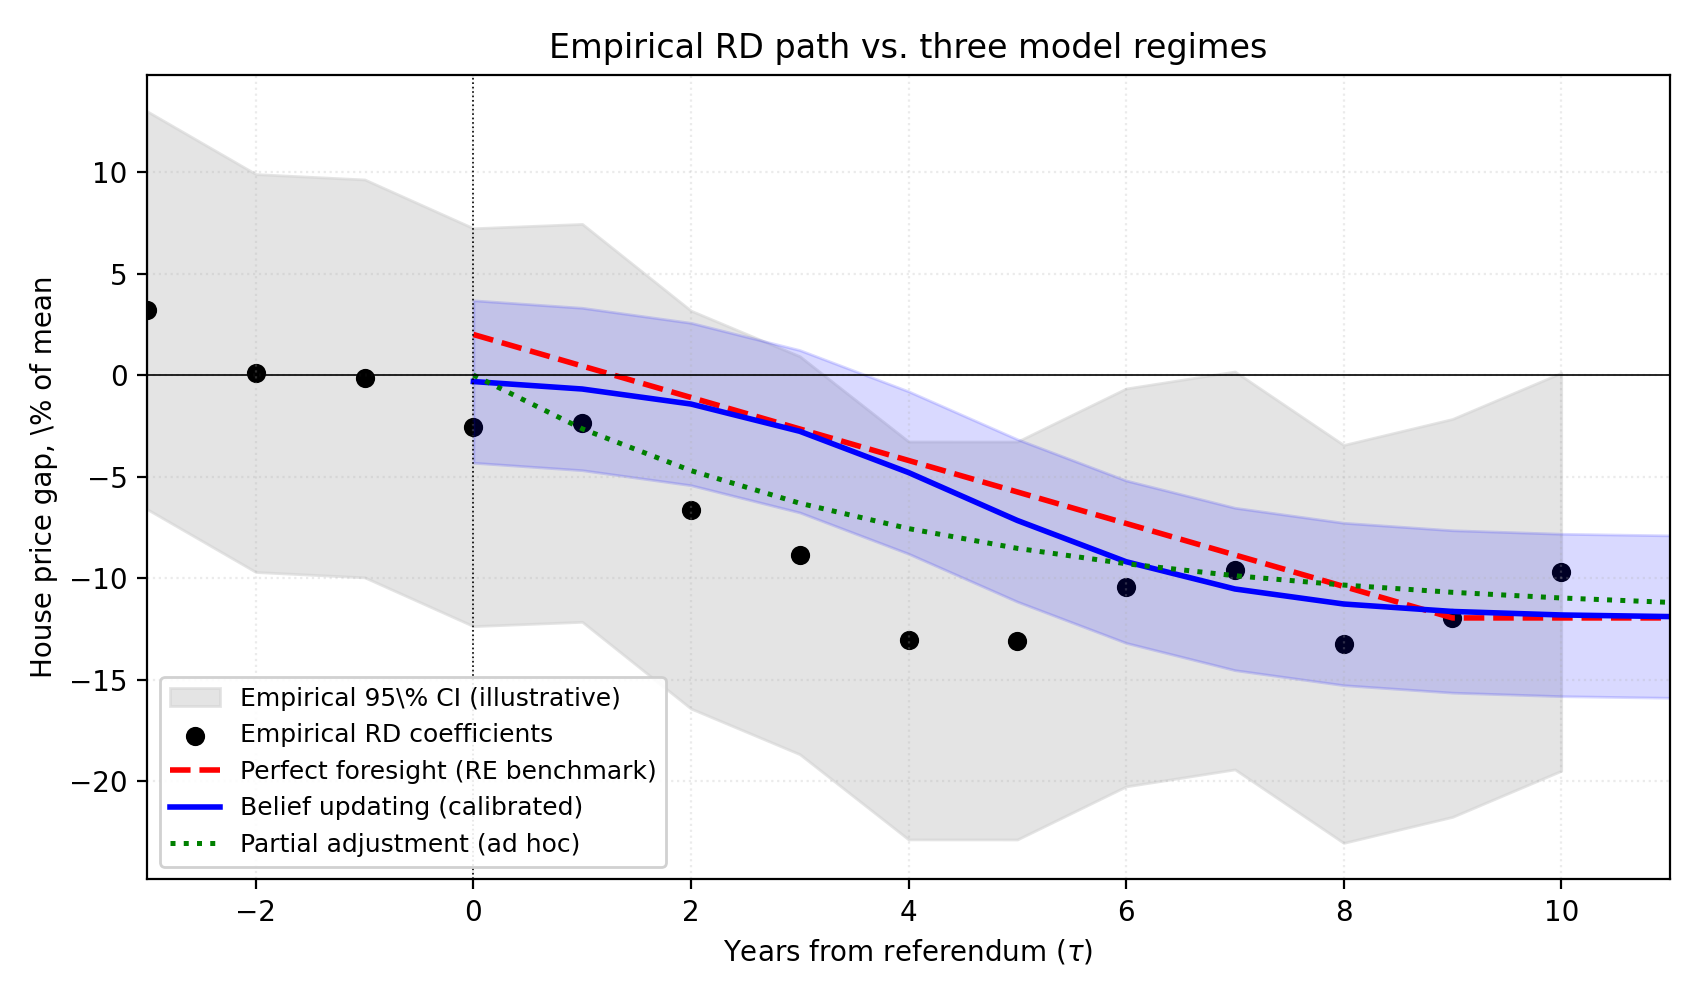
\includegraphics[width=0.9\textwidth]{images/model_vs_data_re_vs_bu.png}
    \caption{Three model paths against empirical house-price RD coefficients. {\it Perfect foresight (RE benchmark, red dashed):} the marginal buyer at $\tau = 0$ instantaneously prices both the immediate tax-cut benefit (which raises the housing-user-cost multiplier $\beta/(1-\beta(1-\delta_h-\tau_h))$ and pushes the price gap up by $\sim 2$\%) and the present value of the subsequent amenity decline (which pushes the gap monotonically downward). The RE benchmark therefore predicts a positive contemporaneous price gap at $\tau = 0$, declining through zero around $\tau = 3$ and settling at the long-run level. This pattern --- a positive bump followed by gradual decline --- is decisively rejected by the empirical RD coefficients in the $\tau \in [0, 2]$ window. {\it Belief updating (blue solid):} under attention frictions / signal extraction on the buyer side, neither the tax-cut benefit nor the future amenity decline is processed at $\tau = 0$; the posterior $\hat{G}_t$ remains anchored at baseline until the road-quality signal sharpens. The price gap is approximately zero through $\tau = 3$ and opens sharply between $\tau = 4$ and $\tau = 9$ as visible decay triggers Bayesian updating. {\it Partial adjustment (dotted):} qualitatively similar to belief updating but lacks an economic primitive to discipline its smoothing parameter. Figure generated by \texttt{code/belief\_updating\_kalman.py}.}
    \label{fig:model_vs_data_re_vs_bu}
\end{figure}

\paragraph{Discussion.}
The belief-updating microfoundation accomplishes three things relative to the original partial-adjustment treatment. First, it provides an economic primitive ($\bar{\sigma}$) whose value is identified from the data and disciplined by a single, transparent moment. Second, it nests the rational-expectations benchmark as a knife-edge restriction, so the test of $\bar{\sigma} = 0$ becomes the structural counterpart to the RE-rejection test of Section \ref{sec:fiscal_illusion}. Third, it generates pre-specified cross-sectional implications --- on urban-rural and price-quantile margins --- that match the reduced-form evidence without requiring additional free parameters.

A natural concern is whether the same dynamics could be generated by purely rational expectations augmented with adjustment costs in housing transactions. Appendix \ref{sec:appxdmodel} reports a sensitivity exercise in which a housing-illiquidity cost is added to the PF specification while $\bar{\sigma}$ is held at zero. The result is a sluggish but {\it monotone} price decline that does not reproduce the empirically-observed near-zero response over $\tau \in [0,3]$ followed by a sharp opening at $\tau = 4$. The kinked, visibility-synchronized profile is a distinctive prediction of the belief-updating mechanism.